\documentclass{article}

\usepackage[usenames,dvipsnames]{color}
\usepackage{graphicx}
\usepackage{bytefield}
\usepackage{hyperref}

\definecolor{lightgray}{gray}{0.8}
\definecolor{lightblue}{rgb}{0.92,0.92,1.0}
\definecolor{lightred}{rgb}{1.0,0.92,0.92}

\newcommand{\rcolor}{lightblue}
\newcommand{\wcolor}{lightred}
\newcommand{\reserved}{lightgray}

\newenvironment{packed_itemize}{
\begin{itemize}
  \setlength{\itemsep}{1pt}
  \setlength{\parskip}{0pt}
  \setlength{\parsep}{0pt}
}{\end{itemize}}

\hypersetup{
    bookmarks=true,         % show bookmarks bar?
    unicode=false,          % non-Latin characters in Acrobat’s bookmarks
    pdftoolbar=true,        % show Acrobat’s toolbar?
    pdfmenubar=true,        % show Acrobat’s menu?
    pdffitwindow=false,     % window fit to page when opened
    pdfstartview={FitH},    % fits the width of the page to the window
    pdftitle={My title},    % title
    pdfauthor={Author},     % author
    pdfsubject={Subject},   % subject of the document
    pdfcreator={Creator},   % creator of the document
    pdfproducer={Producer}, % producer of the document
    pdfkeywords={keyword1} {key2} {key3}, % list of keywords
    pdfnewwindow=true,      % links in new window
    colorlinks=true,        % false: boxed links; true: colored links
    linkcolor=black,        % color of internal links
    citecolor=green,        % color of links to bibliography
    filecolor=magenta,      % color of file links
    urlcolor=cyan           % color of external links
}

\newcommand{\colorbitbox}[4][lrtb]{%
  \bitbox{0}{}%
  \rlap{\bitbox[#1]{#3}{\color{#2}\rule{\width}{\height}}}%
  \bitbox[#1]{#3}{#4}}
\newcommand{\colorwordbox}[4][lrtb]{%
  \bitbox{0}{}%
  \rlap{\wordbox[#1]{#3}{\color{#2}\rule{\width}{\height}}}%
  \wordbox[#1]{#3}{#4}}

\begin{document}

\begin{abstract}
Peanuts are tasty.
\end{abstract}

\section{Overview}

Programmable hardware is increasingly deployed in large, physically distributed control systems.
Hard real-time systems especially benefit from the determinism and low latency of purpose-built hardware.
As reconfigurable hardware components replace traditional software-based systems, 
those hardware components must often communicate directly, over longer distances.
While traditional protocols like CORBA and SOAP 
provide an excellent abstraction for software-to-software communication,
they are a poor fit for hardware-to-hardware communication.
Hardware components typically transfer information in read/write bus cycles
as opposed to the procedure calling interfaces seen in software.

The Etherbone protocol takes an existing bus standard (Wishbone~\cite{wishbone}) 
and extends this bus to run over the network.
A concrete bus standard was chosen, 
because different bus protocols often differ enough that conversion reduces fidelity.
Wishbone was chosen because it is an open standard, simple, and pipe\-lining.
The underlying transport protocol is left open,
as Etherbone's require\-ments are easily met.
This specification defines Etherbone for UDP and TCP.

Etherbone's key features are:
\begin{packed_itemize}
\item Bus-cycle interface
\item Deterministic latency
\item Simple hardware implementation
\item Cut-through/wormhole operation
\item Compatible with software implementations
\item Separate config/control address space
\item Negotiable bus/address widths
\end{packed_itemize}

Etherbone leaves these issues to the lower transport layer:
\begin{packed_itemize}
\item Exactly once delivery (TCP or reliable layer 2)
\item Cut-through switching
\item Authentication (physical access or TLS)
\item Confidentiality
\end{packed_itemize}

%Etherbone was built for use by the GSI/FAIR and CERN/LHC particle accelerator projects.
%Thus, it is used in control systems which span approximately 2 and 20 kilometres respectively.
%As a companion to the WhiteRabbit project~\cite{white-rabbit}, it runs over Gigabit ethernet.
%Assuming fiber optics, the flight times are 10$\mu$s and 100$\mu$s,
%while buffering a 1500-byte Ethernet frame takes 12$\mu$s.

Etherbone was designed for the following use cases:
\begin{packed_itemize}
\item High-precision system control
\item Sensor data acquisition
\item System diagnostics
\item Remote debugging
\item Distributed bus bridging
\end{packed_itemize}

%\section{Related Work}

% RMAP spacewire ESA
%  specific transport
%  unspecified bus protocol
% RDMA for large transfers in HPC (infiband, ethernet and tcp/ip)

\section{Architecture}

Etherbone (EB) connects two Wishbone (WB) buses together as shown in
Figure~\ref{fig:hw-system}.
The WB Intercon is a local bus, for example a crossbar interconnect.
When a WB master wishes to write to a remote slave, 
it writes to the EB bridge,
which is a local WB slave.
The bridge, acting as an EB master, 
translates the request into an EB frame
(Section~\ref{sec:packet-format}) and routes it to
the receiving EB slave.
That slave decodes the request and executes the write over Wishbone.
Finally, the WB interconnect routes the write to the correct slave.

\begin{figure}[t]
\centering%
\includegraphics[width=\columnwidth]{system}
\caption{Etherbone system in hardware}
\label{fig:hw-system}
\end{figure}

Either or both of the devices in Figure~\ref{fig:hw-system} may be replaced by software,
as shown in Figure~\ref{fig:sw-system}.
In this scenario,
the operating system buffers and sends Etherbone frames as requested by the
Etherbone software library.
Client applications may use this library for remote access to
any slave attached to an Etherbone equipped wishbone bus.
This facilitates such tasks as debugging, firmware updates, and monitoring from a
dekstop system.
Applications may also attach devices to a virtual wishbone bus,
perhaps to capture bus cycles or trigger an alarm.
These virtual devices may be mapped into the Wishbone bus of other Etherbone nodes,
hardware or software.

\begin{figure}[t]
\centering%
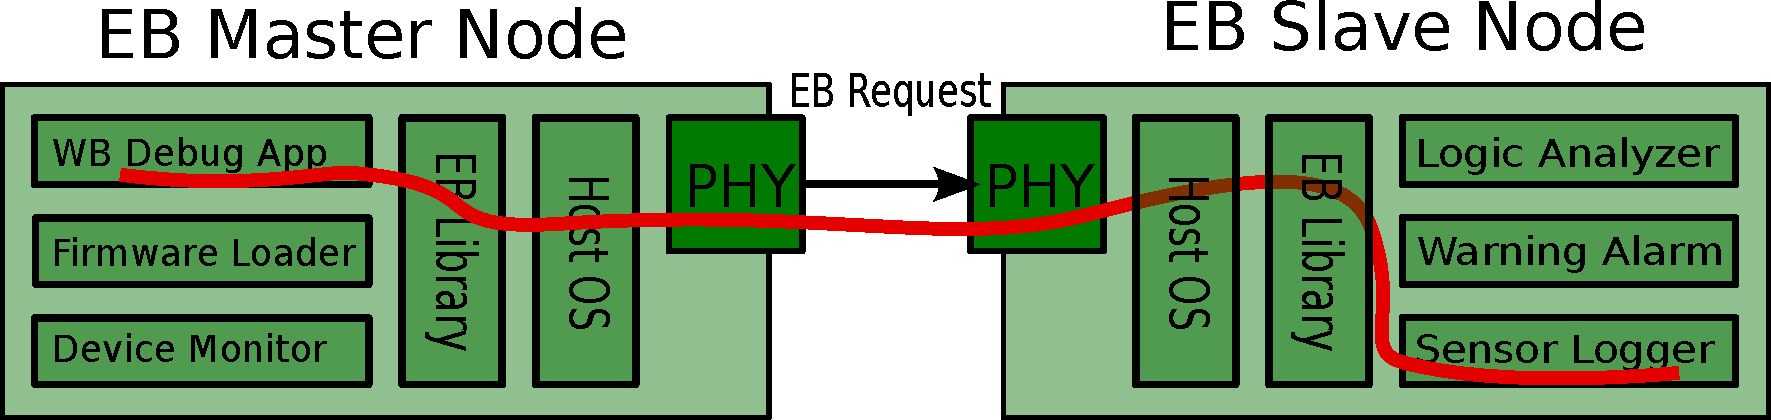
\includegraphics[width=\columnwidth]{software}
\caption{Etherbone system in software}
\label{fig:sw-system}
\end{figure}

\subsection{Addressing}

Slaves on a Wishbone bus have a mapped address range.
Masters read and write to an address on the local bus
and the Intercon routes the operation to the matching slave device.
However, with the introduction of Etherbone, 
there are now multiple reachable Wishbone buses in the facility-wide system.
To select the destination slave, additional address information is required.

When using the software interface,
an application acquires a handle object for the remote bus.
Reads and writes are then performed via the handle object,
requiring only the WB bus address per operation.
To acquire the handle object, 
the application supplies the hostname and port of the remote WB bus.

For a hardware implementation,
the requests come from a local WB master,
which can only provide a WB bus address.
%The WB protocol provides no As the WB pro Requests cannot carry any additional address information to select the WB bus.
To determine the missing address information,
an EB bridge must infer the destination WB bus 
based only on the local WB address requested.
To achieve this,
the EB bridge establishes a configurable mapping from local WB addresses to
destination hostname:ports and target WB addresses.

For example, 
consider an EB bridge occupying address range 0x1000-0x3000 on the local bus.
There is a remote WB bus available on the the host example.com:3434.
We would like to access the address range 0x100-0x200 on that bus.
Thus, we configure our EB bridge to map this range as 0x2000-0x2100 on the
local bus.
Now, when a WB write on our local bus to address 0x2050 is performed,
the bridge transforms this into an EB write destined for example.com:3434 
at address 0x150.

\subsection{Pipelining}

Unlike a local WB bus, where devices answer in a few clock cycles,
a remote bus accessed via EB has a much high latency.
For a 100MHz bus and a distance of only 20km the difference is
10ns to 100$\mu$s. 
For Internet-scale distances, the latency can easily rise to 100ms.
Therefore, 
an application which only issues a new read/write operation when the previous
operation completes will perform $10^4$ to $10^7$ times slower over EB than direct WB.

EB supports pipelining to overcome this significant performance bottleneck.
Instead of issuing a single operation at a time,
an application/device can issue new operations without waiting
for the previous operation to complete.
The results of the operations will arrive in the same order they were issued.
Whenever new operations do not dependend on still incomplete operations,
this can almost entirely mask the performance lost to remote access.

As an example, considering two application using EB.
The first application is a firmware writing tool that needs to write the
firmware and confirm the firmware was written correctly.
This problem can be readily pipelined; 
the operations have an order requirement (confirmation happens after write),
but the choice of operation to issue does not depend on previous results.
The firmware writer can issue a sequence of WWWW...RRRR... operations
in the pipeline without waiting.
Alternatively, it might also use the sequence WRWRWR... to confirm each word
immediately after writing it.
In both cases, the application can issue all of the operations without waiting.
This would not be possible if the application were to iterate a remote function.
Suppose the application wants to compute $f(f(f(...f(x)...)))$ 
using a remote WB slave to calculate function $f$.
Here, the aplication writes $x$ to the remote slave and reads back
$y = f(x)$.
Then the application writes $y$ to the remote slave and reads back
$z = f(y)$.
The write pattern WRWRWR... is the same as the firmware loader,
but here we can only pipeline a single write-read operation pair together.
Until we have received the result $f(x)$, we cannot issue $f(y)$.

In Wishbone, several operations can be grouped into a single bus cycle.
A particularly bad situation that can occur is when dependencies appear within a WB cycle.
Generally, WB cycles acquire the device for use until cycle completion.
On a local bus, any access pattern will work, 
as the operations will complete quickly and release the cycle line.
However, when this happens with EB-sized latencies, 
a cycle might tie up a device for potentially unacceptable duration.
Consider for example a WB cycle that reads from one address 
and writes the result to another address.
Locally, there is no problem; the entire WB cycles executes in a few
nanoseconds.
However, when that same access pattern runs over the network,
the slave device needs to wait for the read result to travel to the master and the final write to travel back.
A very bad design.

Dealing with data dependencies within a cycle is a major complication
addressed in the different implementation options described in
Section~\ref{sec:eb-master}.

\subsection{Config Space}

In addition to remote bus access, 
Etherbone also provides a configuration space.
This config space is used to specify transmission parameters,
recover bus error status codes,
and match read results to the requests.

The config space is an complementary 16-bit wide address space attached to every EB slave.
EB requests can read/write to this configuration space in addition the the normal WB bus.
The config space is divided up into two regions: the register space and the implementation space.
All addresses in the register space correspond to EB control registers,
specified in this document.
The register space spans addresses 0x0-0x7FFF.
The implementation space is guaranteed to be free for whatever use
a hardware/software implementation chooses.
The implementation space spans 0x8000-0xFFFF.

Two important registers in the address space include the error status
register, which reports WB error status codes, and the WB device map pointer,
which provides information about the slaves attached to a remote bus.
The implementation space is typically used by an EB master to receive
the data which it read.
Reads to an EB device trigger a write back to the source EB device.
Those writebacks are often sent to the implementation space 
where they can be handled by the EB core/code and invisible to the WB bus.

\subsection{Bus Widths}

In Wishbone, 
a bus may have a port width that is 8/16/32/64 bits wide.
Thus, a master in one WB bus might write 32-bits at a time,
while a slave in another WB bus expects 16-bits at a time.
Etherbone makes no attempt to convert between differing port widths,
because converting a 32-bit write into two 16-bit writes might change semantics.

However, 
Etherbone does negotiate which port widths are acceptable to both devices.
This mostly affects software,
which can meaningfully support access with different port widths.
Hardware implementations will typically advertise and accept only one width.

Address spaces in WB are conceptually infinite, 
but in practice are constrained to a fixed width.
Address width conversion, as oppposed to port width conversion,
is relatively straight-forward.
Address 0x0400 is that same as 0x00000400.
If a 32-bit device is accessed by a 16-bit device,
the 16-bit device can only see the low 16-bits of the larger device's address space.

Address width is negotiated by Etherbone simply to determine the amount of
space to reserve for message exchanges.
A hardware implementation is free to only advertise address widths
whose message alignment is convenient to them.

\section{Real-time Deployment}
\label{sec:deployment}

One of the key features of Etherbone is that it can used with hard realtime constraints
and extremely low latency.
In this scenario, Etherbone only forms a small part of the complete system.
To meet deadlines, presumably most components must make timing guarantees.
The Etherbone software library, 
due to its dependency on the host operating system,
cannot guarantee responsiveness.
Therefore, in a hard real-time system,
the software library can be used neither as slave nor master.

Furthermore, 

Beyond those timing requirements imposed externally, 
Etherbone requires attached slave devices to respond quickly.
As detailed in Section~\ref{sec:slave-streaming},
Etherbone slaves can use cut-through request processing to avoid buffering delays.
In this situation, 

\subsection{Multimaster competition}

\subsection{Master-Slave cross-talk}
... master gets his answer in
... but he is also a slave and gets traffic there too
=> must have physically distinct cables 

\subsection{Cut-Through}

\section{Programmer Guide}

\subsection{Software}

\subsection{Hardware}

To be written by Matthias.

\section{Implementation}

\subsection{Pipelined Wishbone}

Etherbone is designed to interact with a Wishbone bus as shown in Figure~\ref{fig:wb-eb}.
In the Wishbone bus, every participant is either a master or a slave.
Only masters may issue requests and only slaves may service them.

A request is either a read or a write and includes the target address.
If the request is a write, it also includes the word to store.
A response includes a success/failure status bit and (if a read) the word read.

In pipelined Wishbone, a master may issue multiple requests without waiting for a response.
Slave devices may stall the master when they are unable to buffer further requests.
This pipelined behaviour is essential for high throughput over a network.
With a typical 125MHz wishbone bus, requests can be issued every 8ns.
Over the network, the round trip latency may exceed 200$\mu$s.
define eb-master/eb-slave
(eb-master is a wb-slave is a network client)
(eb-slave is a wb-master is a network server)

block-diagram

streaming


\section{Message Format}

\begin{figure}[t]
 \centering
 \begin{bytefield}{32}
  \bitheader{0,3,4,16,19,20,24,28,32} \\
  \bitbox{16}{\nameref{field:Magic} (0x4E6F)}  &
  \bitbox{4}{\nameref{field:Version}} &
  \colorbitbox{\reserved}{3}{} &
  \bitbox{1}{\rotatebox{90}{\small \nameref{field:PF}}} &
  \bitbox{4}{\nameref{field:AddrSz}} &
  \bitbox{4}{\nameref{field:PortSz}} \\
  \wordgroupl{\rotatebox{90}{WB Cycle (Repeats)}}
   \colorbitbox{\reserved}{3}{} &
   \bitbox{1}{\rotatebox{90}{\small \nameref{field:RF}}}&
   \bitbox{12}{\nameref{field:RCount}} &
   \colorbitbox{\reserved}{3}{} &
   \bitbox{1}{\rotatebox{90}{\small \nameref{field:WF}}} &
   \bitbox{12}{\nameref{field:WCount}} \\
   \wordgroupr{\rotatebox{270}{\nameref{field:RCount} $\not= 0$}}
    \colorwordbox{\rcolor}{1}{\nameref{field:BaseRetAddr}} \\
    \colorwordbox{\rcolor}{1}{\nameref{field:ReadAddr} 1} \\
    \colorwordbox{\rcolor}{1}{\nameref{field:ReadAddr} 2} \\
    \colorwordbox[tb]{\rcolor}{1}{$\vdots$ \\[1ex]} \\
    \colorwordbox{\rcolor}{1}{\nameref{field:ReadAddr} $N$}
   \endwordgroupr \\
   \wordgroupr{\rotatebox{270}{WCount $\not= 0$}}
    \colorwordbox{\wcolor}{1}{\nameref{field:BaseWriteAddr}} \\
    \colorwordbox{\wcolor}{1}{\nameref{field:WriteVal} 1} \\
    \colorwordbox{\wcolor}{1}{\nameref{field:WriteVal} 2} \\
    \colorwordbox[tb]{\wcolor}{1}{$\vdots$ \\[1ex]} \\
    \colorwordbox{\wcolor}{1}{\nameref{field:WriteVal} $N$}
   \endwordgroupr 
  \endwordgroupl \\
 \end{bytefield}
 \caption{Etherbone Message Format}
 \label{fig:header}
\end{figure}

\section{Config Registers}

\begin{tabular}{


\subsection{Server Operation}
\subsubsection{Buffered}
\subsubsection{Streaming}

\subsection{Client Operation}
\label{sec:eb-master}

\subsubsection{Software - Forbid Spanning}
can enforce this -- don't send until cycle done
\subsubsection{Buffered - Hold High}
unfortunately, cycle line can't drop until acks come
... this approach keeps remote cycle line high (for an entire RTT)
\subsubsection{Buffered - Fast Release}
... this approach speculatively drops the cycle line the moment requests stop coming
\subsubsection{Streaming}

\end{document}

